\documentclass[aspectratio=169,10pt]{beamer}
\usetheme{Madrid}
\usecolortheme{default}

\usepackage[utf8]{inputenc}
\usepackage[T1]{fontenc}
\usepackage{amsmath,amssymb}
\usepackage{booktabs}
\usepackage{graphicx}
\usepackage{tikz}
\usetikzlibrary{shapes,arrows.meta,positioning}
\usepackage{listings}
\usepackage{hyperref}

\definecolor{unibblue}{RGB}{0,51,102}
\definecolor{unibgold}{RGB}{212,175,55}
\definecolor{unibgreen}{RGB}{0,128,0}
\definecolor{codebg}{RGB}{244,247,251}

\setbeamercolor{structure}{fg=unibblue}
\setbeamercolor{palette primary}{bg=unibblue,fg=white}
\setbeamercolor{palette secondary}{bg=unibblue!85,fg=white}
\setbeamercolor{palette tertiary}{bg=unibblue!70,fg=white}
\setbeamercolor{block title}{bg=unibblue!90,fg=white}
\setbeamercolor{block body}{bg=unibblue!8,fg=black}
\setbeamercolor{alertblock title}{bg=unibgold!90,fg=black}
\setbeamercolor{alertblock body}{bg=unibgold!14,fg=black}
\setbeamercolor{exampleblock title}{bg=unibgreen!85,fg=white}
\setbeamercolor{exampleblock body}{bg=unibgreen!8,fg=black}

\title[Aliran Daya Python — Modul 2]{Analisis Aliran Daya Menggunakan Python}
\subtitle{Modul 2: Algoritma Numerik Aliran Daya \textit{From-Scratch} (NR, Q-Limit, FDLF \& GS)}
\author[Novalio Daratha]{Novalio Daratha\\Program Studi Teknik Elektro, Universitas Bengkulu}
\date{Workshop Teknis Intensif (32 JP) — 2026}

\begin{document}

\begin{frame}
  \titlepage
\end{frame}

\begin{frame}{Agenda Modul 2 (8 JP)}
  \tableofcontents
\end{frame}

\section{Formulasi Polar Newton-Raphson}

\begin{frame}{Persamaan Aliran Daya Polar \& Vektor Mismatch}
  \begin{block}{Injeksi Daya Aktif \& Reaktif pada Bus $i$}
    \begin{align*}
      P_i(\boldsymbol{\theta}, |\mathbf{V}|) &= |V_i|\sum_{k=1}^{N_b} |V_k|\left(G_{ik}\cos\theta_{ik} + B_{ik}\sin\theta_{ik}\right) \\
      Q_i(\boldsymbol{\theta}, |\mathbf{V}|) &= |V_i|\sum_{k=1}^{N_b} |V_k|\left(G_{ik}\sin\theta_{ik} - B_{ik}\cos\theta_{ik}\right)
    \end{align*}
  \end{block}
  \begin{columns}[T]
    \begin{column}{0.52\textwidth}
      \begin{exampleblock}{Persamaan Koreksi Newton-Raphson}
        \[
          \begin{bmatrix} \mathbf{H} & \mathbf{N} \\ \mathbf{M} & \mathbf{L} \end{bmatrix}
          \begin{bmatrix} \Delta\boldsymbol{\theta}_{\mathcal{PV}\cup\mathcal{PQ}} \\ \Delta|\mathbf{V}|_{\mathcal{PQ}} \end{bmatrix}
          =
          \begin{bmatrix} \mathbf{P}^{\text{sch}} - \mathbf{P}^{\text{calc}} \\ \mathbf{Q}^{\text{sch}} - \mathbf{Q}^{\text{calc}} \end{bmatrix}
        \]
      \end{exampleblock}
    \end{column}
    \begin{column}{0.45\textwidth}
      \begin{alertblock}{Dimensi Sistem ($n$)}
        $n = N_{\text{PV}} + 2 N_{\text{PQ}}$.\\
        Pada IEEE 14-Bus (1 Slack, 4 PV, 9 PQ):\\
        $n = 4 + 2(9) = \mathbf{22 \times 22}$.
      \end{alertblock}
    \end{column}
  \end{columns}
\end{frame}

\section{Matriks Jacobian Polar Lengkap}

\begin{frame}{Empat Sub-Matriks Jacobian Polar ($J_1, J_2, J_3, J_4$)}
  \scriptsize
  \begin{center}
  \begin{tabular}{@{}lll@{}}
    \toprule
    \textbf{Blok Jacobian} & \textbf{Off-Diagonal ($i \neq k$)} & \textbf{Diagonal ($i = k$)} \\
    \midrule
    $J_1 = H_{ik} = \dfrac{\partial P_i}{\partial \theta_k}$ & $|V_i||V_k|(G_{ik}\sin\theta_{ik} - B_{ik}\cos\theta_{ik})$ & $-Q_i - B_{ii}|V_i|^2$ \\[7pt]
    $J_2 = N_{ik} = \dfrac{\partial P_i}{\partial |V_k|}$ & $|V_i|(G_{ik}\cos\theta_{ik} + B_{ik}\sin\theta_{ik})$ & $\dfrac{P_i}{|V_i|} + G_{ii}|V_i|$ \\[7pt]
    $J_3 = M_{ik} = \dfrac{\partial Q_i}{\partial \theta_k}$ & $-|V_i||V_k|(G_{ik}\cos\theta_{ik} + B_{ik}\sin\theta_{ik})$ & $P_i - G_{ii}|V_i|^2$ \\[7pt]
    $J_4 = L_{ik} = \dfrac{\partial Q_i}{\partial |V_k|}$ & $|V_i|(G_{ik}\sin\theta_{ik} - B_{ik}\cos\theta_{ik})$ & $\dfrac{Q_i}{|V_i|} - B_{ii}|V_i|$ \\
    \bottomrule
  \end{tabular}
  \end{center}
  \normalsize
  \vspace{0.2cm}
  \begin{block}{Bentuk Matriks Kompleks Tervektorisasi (\texttt{newton\_raphson.py})}
    $\dfrac{\partial \mathbf{S}}{\partial \boldsymbol{\theta}} = j\,\operatorname{diag}(\mathbf{V})\left(\operatorname{diag}(\mathbf{I}) - Y_{\text{bus}}\operatorname{diag}(\mathbf{V})\right)^*$, \quad
    $\dfrac{\partial \mathbf{S}}{\partial |\mathbf{V}|} = \operatorname{diag}(\mathbf{V})\left(Y_{\text{bus}}\operatorname{diag}(\bar{\mathbf{V}})\right)^* + \operatorname{diag}(\mathbf{I})^*\operatorname{diag}(\bar{\mathbf{V}})$
  \end{block}
\end{frame}

\section{Penegakan Batas Reaktif ($Q$-Limit) \& Robustnes}

\begin{frame}{Mekanisme \textit{Q-Limit Switching} ($PV \leftrightarrow PQ$) Berbasis AVR}
  \begin{columns}[T]
    \begin{column}{0.53\textwidth}
      \begin{center}
        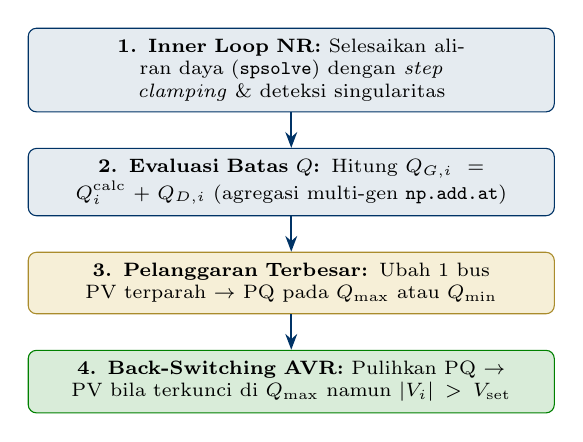
\begin{tikzpicture}[
          node distance=0.45cm,
          box/.style={draw=unibblue, fill=unibblue!10, rounded corners=3pt, text width=6.4cm, align=center, font=\scriptsize, inner sep=4pt},
          arr/.style={-{Stealth[length=2mm]}, thick, color=unibblue}
        ]
          \node[box] (s1) {\textbf{1. Inner Loop NR:} Selesaikan aliran daya (\texttt{spsolve}) dengan \textit{step clamping} \& deteksi singularitas};
          \node[box, below=of s1] (s2) {\textbf{2. Evaluasi Batas $Q$:} Hitung $Q_{G,i} = Q_i^{\text{calc}} + Q_{D,i}$ (agregasi multi-gen \texttt{np.add.at})};
          \node[box, below=of s2, fill=unibgold!20, draw=unibgold!80!black] (s3) {\textbf{3. Pelanggaran Terbesar:} Ubah 1 bus PV terparah $\to$ PQ pada $Q_{\max}$ atau $Q_{\min}$};
          \node[box, below=of s3, fill=unibgreen!15, draw=unibgreen] (s4) {\textbf{4. Back-Switching AVR:} Pulihkan PQ $\to$ PV bila terkunci di $Q_{\max}$ namun $|V_i| > V_{\text{set}}$};
          \draw[arr] (s1) -- (s2);
          \draw[arr] (s2) -- (s3);
          \draw[arr] (s3) -- (s4);
        \end{tikzpicture}
      \end{center}
    \end{column}
    \begin{column}{0.44\textwidth}
      \begin{exampleblock}{Eksperimen Lab 2.4 (Bus 8)}
        Menurunkan $Q_{\max,8} = 10\text{ MVAr}$ memicu peralihan Bus 8 dari PV $\to$ PQ:
        \begin{itemize}
          \item $|V_8|$ turun: $1{,}0900 \to \mathbf{1{,}0675\text{ p.u.}}$
          \item Dimensi Jacobian naik: $22 \to 23$
          \item Konvergen tuntas dalam 2 \textit{outer loop}.
        \end{itemize}
      \end{exampleblock}
      \begin{alertblock}{Penanganan Jaringan Sakit}
        Gunakan \texttt{MatrixRankWarning}, cek \texttt{NaN/Inf}, dan \textit{clamping} $|\Delta\theta|, |\Delta|V||$.
      \end{alertblock}
    \end{column}
  \end{columns}
\end{frame}

\section{Perbandingan NR vs FDLF vs Gauss-Seidel}

\begin{frame}{Perbandingan Laju Konvergensi pada IEEE 14-Bus ($\varepsilon = 10^{-8}$)}
  \begin{columns}[T]
    \begin{column}{0.55\textwidth}
      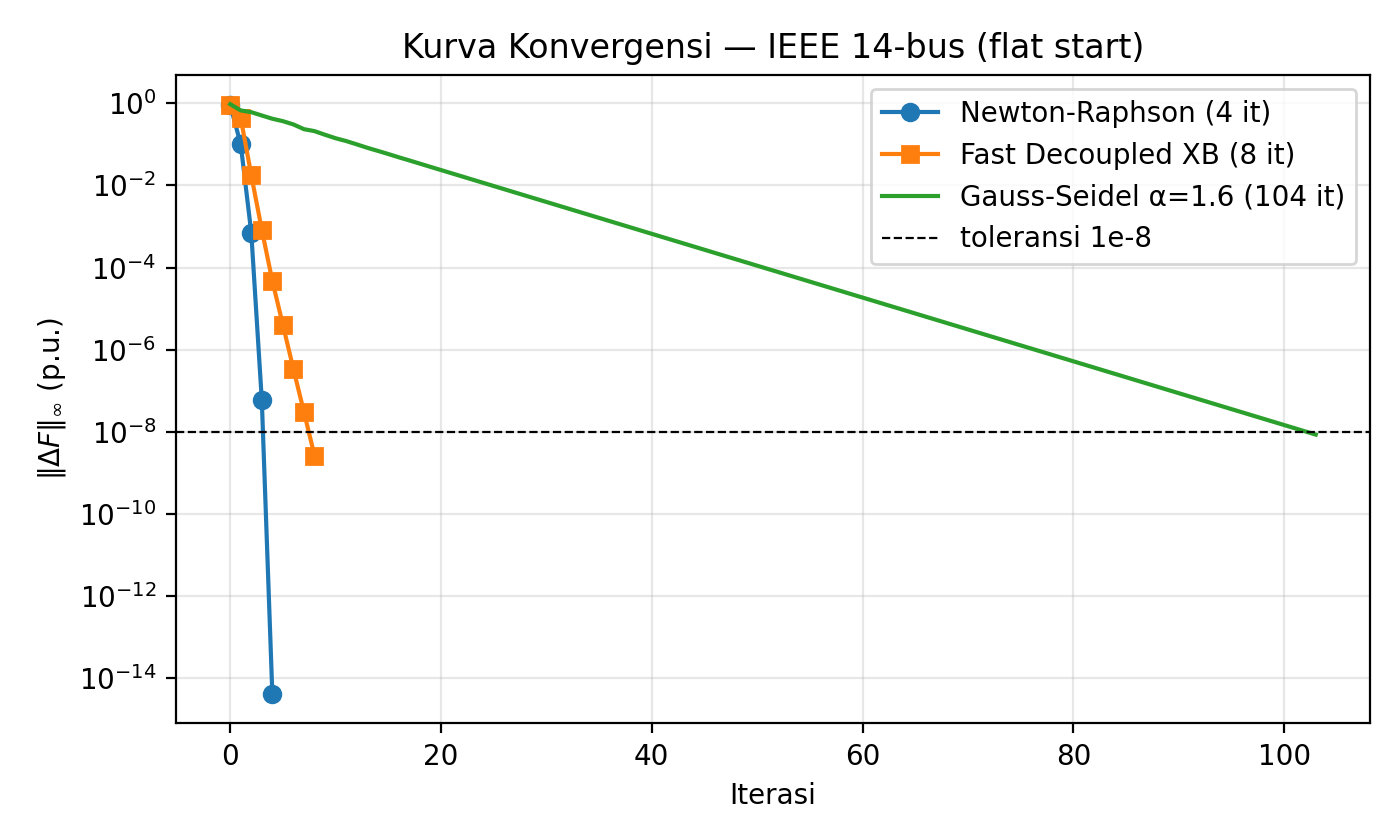
\includegraphics[width=\textwidth]{../figures/konvergensi.png}
    \end{column}
    \begin{column}{0.43\textwidth}
      \scriptsize
      \begin{tabular}{@{}lcc@{}}
        \toprule
        \textbf{Metode} & \textbf{Iterasi} & \textbf{Orde} \\
        \midrule
        Newton-Raphson & \textbf{4} & Kuadratik \\
        FDLF (Skema XB) & 8 & Linear cepat \\
        Gauss-Seidel ($\alpha=1{,}6$) & 104 & Linear lambat \\
        \bottomrule
      \end{tabular}
      \vspace{0.25cm}
      \normalsize
      \begin{block}{Jejak Mismatch NR}
        \scriptsize
        Iter 0: $9{,}22\times 10^{-1}$\\
        Iter 1: $1{,}01\times 10^{-1}$\\
        Iter 2: $7{,}10\times 10^{-4}$\\
        Iter 3: $5{,}98\times 10^{-8}$\\
        Iter 4: $4{,}15\times 10^{-15}\text{ p.u.}$
      \end{block}
      \begin{alertblock}{Sensitivitas Rasio $R/X$}
        Jika $R \times 3$, FDLF melambat drastis karena kopling $J_2, J_3$ tidak lagi dapat diabaikan.
      \end{alertblock}
    \end{column}
  \end{columns}
\end{frame}

\begin{frame}{Terima Kasih — Lanjut ke Modul 3}
  \begin{center}
    \vspace{0.8cm}
    {\Large \textbf{Terima Kasih}}\\
    \vspace{0.4cm}
    {\large Sesi Tanya Jawab \& Praktikum \texttt{python3 newton\_raphson.py}}\\
    \vspace{1.2cm}
    Novalio Daratha\\
    Program Studi Teknik Elektro, Universitas Bengkulu\\
    \texttt{https://ndaratha.my.id/w-pf/}
  \end{center}
\end{frame}

\end{document}
